\documentclass[12pt, draftcls, onecolumn]{IEEEtran}
\makeatletter
\def\subsubsection{\@startsection{subsubsection}{3}{\z@}{0ex plus 0.1ex minus 0.1ex}{0ex}{\normalfont\normalsize\bfseries}}
\makeatother
\usepackage[T1]{fontenc}
\usepackage{subfigure}
\usepackage{ulem}
\usepackage{amsmath}
\allowdisplaybreaks
\usepackage{hhline}
\usepackage{yfonts,color}
\usepackage{soul,xcolor}
\usepackage{verbatim}
\usepackage{amsmath}
\allowdisplaybreaks
\usepackage{amssymb}
\usepackage{amsthm}
\usepackage{float}
\usepackage{bm}
\usepackage{url}
\usepackage{array}
\usepackage{cite}
\usepackage{graphicx}
\usepackage{framed}
\usepackage{balance}
\usepackage{epsfig,epstopdf}
\usepackage{booktabs}
\usepackage{courier}
\usepackage{subfigure}
\usepackage{pseudocode}
\usepackage{enumerate}
\usepackage{algorithm}
\usepackage{algpseudocode}
\newtheorem{definition}{Definition}
\newtheorem{theorem}{Theorem}
\newtheorem{lemma}[theorem]{Lemma}
\newtheorem{proposition}[theorem]{Proposition}
\newtheorem{corollary}[theorem]{Corollary}
\newtheorem{assumption}{Assumption}
\newtheorem{remark}{Remark}
\renewcommand{\algorithmicrequire}{\textbf{Initialization:}}
\renewcommand{\algorithmicensure}{\textbf{Output:}}
\newcommand{\rom}[1]{\uppercase\expandafter{\romannumeral #1\relax}}
\usepackage{color}
\usepackage{soul,xcolor}
\newcommand{\nm}[1]{{\color{blue}\text{\bf{[NM: #1]}}}}
\newcommand{\sst}[1]{\st{#1}}
\newcommand{\gs}[1]{{\color{orange}\bf{[GS: #1]}}}
\newcommand{\remove}[1]{{\color{magenta}{\bf REMOVE: [#1]}}}
\newcommand{\add}[1]{{\color{red}{#1}}}
\newcommand{\ull}[1]{\textbf{\color{red}\ul{#1}}}
\normalem
\begin{document} 
\setulcolor{red}
\setul{red}{2pt}
\title{PU Occupancy Behavior Estimation}
\author{Bharath Keshavamurthy and Nicol\`{o} Michelusi
\thanks{Keshavamurthy and Michelusi are with the School of Electrical and Computer Engineering, Purdue University, West Lafayette, IN, USA; emails:<bkeshava,michelus>@purdue.edu.}}
\maketitle
\setstcolor{red}
\maketitle
\section{Static PU with Channel Correlation and Complete Information}
\subsection{Assumptions}
\begin{enumerate}
    \item There's only one Primary User (PU) in the wideband spectrum of interest.
    \item There's only one Secondary User (SU) making observations of the PU occupancy in the wideband spectrum of interest.
    \item If $B\ =\ \{b_1,\ b_2,\ b_3,\ .....,\ b_K\}$ represents the set of all sub-bands in the wideband spectrum of interest, then it's assumed that considering energy detection, for any band $b_k\ \in\ B$, $E[|X_k(i)|^2]\ =\ 1$ if it is occupied by the PU, else $E[|X_k(i)|^2]\ =\ 0$.
    \item The noise samples $V_k(i)$ are i.i.d Complex Gaussian with zero mean and variance $\sigma_V^2$ independent of PU occupancy state in the wideband spectrum of interest. Furthermore, the noise samples are i.i.d across frequency and across observation rounds.
    \item Furthermore, the PU occupancy behavior is assumed to be static during the estimation period of our algorithm.
    \item The Hidden Markov Model parameters are assumed to be known for now in order to come up with an optimal algorithm for state estimation.
\end{enumerate}
\subsection{Observation Model}
\begin{equation}\label{1}
    y(n) = \sum_{m=0}^{M-1} h(m)x(n-m) + v(n)
\end{equation}
Here, $y(n)$ is the wideband signal observed at the SU receiver expressed as a convolution of the PU signal $x(n)$ with the channel impulse response $h(n)$ added with a noise term v(n).
Equation (\ref{1}) can be written in the frequency domain by taking a K-point DFT which decomposes the observed wideband signal into K discrete narrow-band components as shown below,
\begin{equation}\label{2}
    Y_k(i) = H_kX_k(i) + V_k(i)
\end{equation}
where,
\\$i\ \in\ \{1,\ 2,\ 3,\ .........,\ T\}$ represents the index of the observation
\\\textbf{NOTE}: Multiple observations of all the frequency bands are made by the SU for training the algorithm and averaging the results over numerous iterations. However, the PU occupancy behavior in this case remains static over time.
\\$k\ \in\ \{1,\ 2,\ 3,\ .........,\ K\}$ represents the index of the sub-band
\\$V_k(i)\ \sim\ \mathcal{N}(0,\ \sigma_V^2)$ represents the zero-mean additive Gaussian noise sample
\\$H_k\ \sim\ \mathcal{N}(0,\ \sigma_H^2)$ represents the $k^{th}$ DFT coefficient of the impulse response $h(n)$ of the channel in between the PU and the SU receiver
\\The PU occupancy behavior in each sub-band $b_k\ \in\ B$ is modelled as $X_k$ taking two possible values $0\ and\ 1$. Therefore, the PU occupancy behavior in the entire wideband spectrum of interest discretized into narrow-band frequency components can be modelled as a vector of size $|B|\ =\ K$ such that,
\begin{equation}\label{3}
    \vec{X} = [X_1, X_2, X_3, ........., X_K]^T \in \{0,1\}^K
\end{equation}
\subsection{System Model}
The true states encapsulate the actual behavior of the PU which is an unobserved Markov process and the measurements at the SU are noisy observations of the true states which are modelled to be the observed states of a Hidden Markov Model.
For some sub-band $j\ \in\ \{2,\ 3,\ 4,\ .....,\ K\}$, the system is assumed to satisfy the Markov property as shown below,
\[P(X_{j}(i)|X_{j-1}(i),\ X_{j-2}(i),\ .....,\ X_1(i))\ =\ P(X_{j}(i)|X_{j-1}(i)),\ for\ j>1,\]
\[And,\ we\ will\ use\ P(X_1(i))\ for\ j=1.\]
Since \textbf{the PU is assumed to be static in the period of our estimation}, we can write the above assumption as,
\[P(X_{j}|X_{j-1},\ X_{j-2},\ .....,\ X_1)\ =\ P(X_{j}|X_{j-1}),\ for\ j>1,\]
\[And,\ we\ will\ use\ P(X_1)\ for\ j=1.\]
Now, we know that,
\[\vec{X}\ =\ [X_1,\ X_2,\ X_3,\ ......,\ X_K]^T\] which realizes as,
\[\vec{x}\ =\ [x_1,\ x_2,\ x_3,\ ......,\ x_K]^T\]
So,
\begin{equation}\label{4}
    P(\vec{X}=\vec{x}) = P(X_1=x_1) \prod_{k=2}^{K} P(X_k=x_k|X_{k-1}=x_{k-1})
\end{equation}
Now, let's expand on the observation model. With a realization $x_k\ in\ \{0,1\}$ of $X_k$, we have from assumption 3 that,
\[E[|X_k(i)|^2]\ =\ x_k,\ given\ X_k\ during\ observation\ cycle\ i\ has\ realized\ as\ x_k\]
Taking the expectation operator on both sides of equation (\ref{2}) given $X_k$ has realized as $x_k$, we have,
\[E[Y_k(i)\ |\ X_k(i)=x_k]\ =\ E[H_kx_k]\ +\ E[V_k(i)]\]
\[E[Y_k(i)\ |\ X_k(i)=x_k]\ =\ E[H_k]E[x_k]\ +\ E[V_k(i)]\]
\[E[Y_k(i)\ |\ X_k(i)=x_k]\ =\ 0\ +\ 0\]
\begin{equation}\label{5}
    E[Y_k(i) | X_k(i) = x_k] = 0
\end{equation}
because, as already discussed, $V_k(i)\ \sim\ \mathcal{N}(0,\ \sigma_V^2)$ and $H_k\ \sim\ \mathcal{N}(0,\ \sigma_H^2)$.
\\Furthermore, the variance of $Y_k(i)$ given $X_k$ at observation cycle $i$ has realized as $x_k$, is calculated to be, 
\begin{equation*}
    Var[Y_k(i) | X_k(i) = x_k] = E[(Y_k(i) | X_k(i) = x_k)^2] - [E[Y_k(i) | X_k(i) = x_k]]^2
\end{equation*}
\begin{equation*}
    Var[Y_k(i) | X_k(i) = x_k] = E[|H_kX_k(i)|^2 + |V_k(i)|^2 + 2H_kX_k(i)V_k(i)] - (0)^2
\end{equation*}
\begin{equation*}
    Var[Y_k(i) | X_k(i) = x_k] = \sigma_H^2E[|X_k(i)|^2] + \sigma_V^2 + 2E[H_k]E[X_k(i)]E[V_k(i)]
\end{equation*}
\begin{equation}\label{6}
    Var[Y_k(i) | X_k(i) = x_k] = \sigma_H^2x_k + \sigma_V^2
\end{equation}
\subsection{Visualization of Spatially Correlated PU Occupancy Behavior}
The following visualization results illustrate the Occupancy Behavior of the Primary User in a wideband spectrum of interest consisting of 18 frequency bands observed over 100 sampling rounds. The PU behavior is assumed to be static (constant across time).
\begin{itemize}
    \item Figure 1 depicts the PU Occupancy Behavior across time indices (sampling rounds) and across channel indices (frequency bands) assuming that a Markovian correlation exists across the channel indices based on the System Model detailed in the previous subsection. Specifically,
    \[P(Occupied|Idle)\ =\ P(X_j = 1|X_i = 0)\ =\ p\ =\ 0.3\]
    \[P(Occupied)\ =\ P(X_i\ =\ 1)\ =\ \Pi\ =\ 0.6\]
    \item Figure 2 depicts the PU Occupancy Behavior across time indices (sampling rounds) and across channel indices (frequency bands) assuming independence across channels, i.e,
    \[P(Occupied|Idle)\ =\ P(X_j = 1|X_i = 0)\ =\ p\ =\ P(Occupied)\ =\ P(X_i\ =\ 1)\ = \Pi\ =\ 0.3\]
\end{itemize}
\begin{figure}[t]
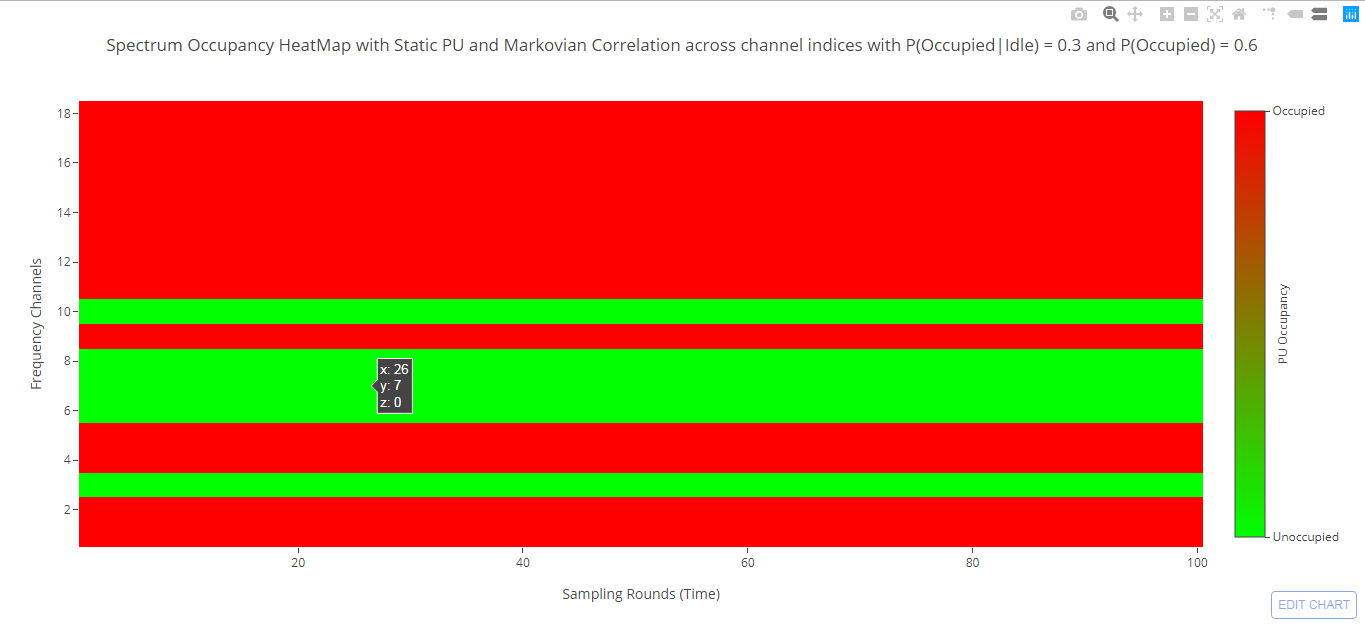
\includegraphics[width=1.0\textwidth]{Spectrum_Occupancy_HeatMap_Static_Spatial_Corr.png}
\caption{Static PU Occupancy Behavior with Markovian Correlation across channel indices}
\label{fig:mesh1}
\centering
\end{figure}
\begin{figure}[t]
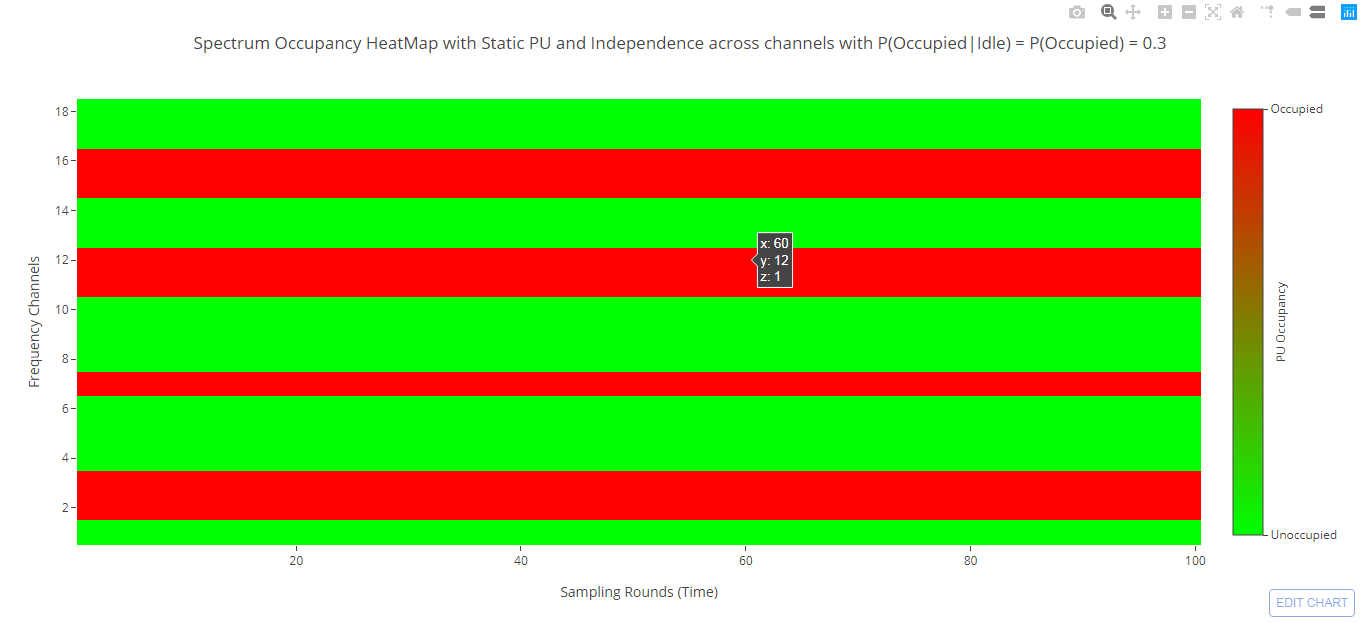
\includegraphics[width=1.0\textwidth]{Spectrum_Occupancy_HeatMap_Static_Independence.png}
\caption{Static PU Occupancy Behavior with independence among channels}
\label{fig:mesh2}
\centering
\end{figure}
\subsection{The Estimator}
\textbf{Given}: The observations of the K frequency sub-bands in the wideband spectrum of interest, i.e. $Y_1,\ Y_2,\ Y_3,\ .....,\ Y_K$
\\\textbf{Assuming} the state transition probability matrix $A$ and the array of initial probabilities $\Pi$ are known.
\\\textbf{From the observation model}, we already know that the emission probabilities are given by,
\[P(Y_k|X_k = x_k)\ \sim \mathcal{N}(0,\ \sigma_H^2x_k+\sigma_V^2)\]
Now, the problem of estimating a sequence of states across the frequency bands in a Hidden Markov Model can be solved using Dynamic Programming to give us the most likely sequence of hidden states called the \textbf{Viterbi Path} based on the sequence of noisy observations of the true states of the frequency sub-bands.
\\From the above statements we can write,
\begin{equation*}
    P(\vec{X}=\vec{x}) = P(X_1=x_1) \prod_{k=2}^{K} P(X_k=x_k|X_{k-1}=x_{k-1})
\end{equation*}
Now, the optimization problem can be written as follows,
\begin{equation}\label{7}
    \vec{x}^* = argmax_{\vec{x}} P(\vec{X}|\vec{Y})
\end{equation}
Here,
$\vec{Y}$ represents the observation vector consisting of the observations of the K sub-bands given by equation (\ref{2}), as shown below,
\[\vec{Y}\ =\ [{Y}_1,\ {Y}_2,\ ....,\ {Y}_K]^T\]
In other words,
\[\vec{x}^*\ represents\ the\ Viterbi\ path\ across\ frequency\ sub-bands\]
\[\vec{Y}\ represents\ the\ sequence\ of\ observations\ across\ frequency\ sub-bands\]
This argmax problem can be re-written as a maximization problem of the joint distribution due to the proportional relation between the joint and the conditional. Therefore, Equation (\ref{7}) can be written as,
\begin{equation}\label{8}
    V_{i}^{(j)}\ =\ max_{x_1,x_2,...,x_{i-1}}P(y_1,y_2,...,y_{i-1},x_1,x_2,...,x_{i-1},y_i,x_{i}=j)
\end{equation}
Here, $V_{i}^{(j)}$ represents \textbf{a value function in our optimization problem tracking the sequence of states of sub-bands that maximize the joint distribution of states and observations as detailed in Equation (\ref{8})}.
\\Now, for the $(i+1)^{th}$ sub-band in state $l$, repeating the same step, we have,
\begin{equation}\label{9}
    V_{i+1}^{(l)}\ =\ max_{x_1,x_2,...,x_i}P(y_1,y_2,...,y_i,x_1,x_2,...,x_i,y_{i+1},x_{i+1}=l)
\end{equation}
Using the definition of conditional probability, we have,
\begin{equation}\label{10}
    V_{i+1}^{(l)}\ =\ max_{x_1,x_2,...,x_i}P(y_{i+1},x_{i+1}=l|y_1,y_2,...,y_i,x_1,x_2,...,x_i)\\P(y_1,y_2,...,y_i,x_1,x_2,...,x_i)
\end{equation}
Now, from the Markov Property, we have,
\begin{equation}\label{11}
    V_{i+1}^{(l)}\ =\ max_{x_1,x_2,...,x_i}P(y_{i+1},x_{i+1}=l|x_i)P(y_1,y_2,...,y_i,x_1,x_2,...,x_i)
\end{equation}
Pushing the maximization operator in,
\begin{equation}\label{12}
    V_{i+1}^{(l)}\ =\ max_{j}[P(y_{i+1},x_{i+1}=l|x_i=j)max_{x_1,x_2,...,x_{i-1}}[P(y_1,y_2,...,y_{i-1},x_1,x_2,...,x_{i-1},y_i,x_i=j)]]
\end{equation}
Using Equation (\ref{8}),
\begin{equation}\label{13}
    V_{i+1}^{(l)}\ =\ max_{j}[P(y_{i+1},x_{i+1}=l|x_i=j)V_i^{(j)}]
\end{equation}
We know that, for three random variables R, U, and W,
\[P(R,U|W)\ =\ P(U|R,W)P(R|W)\]
Using this, we have,
\begin{equation}\label{14}
    V_{i+1}^{(l)}\ =\ max_{j}[P(y_{i+1}|x_{i+1}=l,x_i=j)P(x_{i+1}=l|x_i=j)V_i^{(j)}]
\end{equation}
\begin{equation}\label{15}
    V_{i+1}^{(l)}\ =\ max_{j}[P(y_{i+1}|x_{i+1}=l)P(x_{i+1}=l|x_i=j)V_i^{(j)}]
\end{equation}
Let, $m_l(y_{i+1})$ be the emission probability, i.e. the probability of emission of observation $y_{i+1}$ in state $l$.
\\Let, $a_{jl}$ be the state transition probability.
Then, 
\begin{equation}\label{16}
    V_{i+1}^{(l)}\ =\ m_l(y_{i+1})\ max_{j}[a_{jl}V_i^{(j)}]
\end{equation}
Here, from the observation model,
\[m_l(y_{i+1})\ \sim \mathcal{N}(0,\ \sigma_H^2l+\sigma_V^2)\]
And, from the system's Markov model,
\[a_{jl}\ \in\ A,\ :\ a_{jl}\ =\ P(x_{i+1}=l|x_i=j)\]
Equation (\ref{16}) constitutes the \textbf{Forward Recursion aspect of the Viterbi algorithm}.
\\Now, we analytically derive the \textbf{Backtrack feature of the Viterbi algorithm} below.
\\The state of the $K^{th}$ sub-band, i.e the last state in the Viterbi path is given by,
\begin{equation}\label{17}
    k^*\ =\ argmax_k\ V_K^{(k)}
\end{equation}
This can be written as follows,
\begin{equation}\label{18}
    k^*\ =\ argmax_k\ max_{x_1,x_2,...,x_{K-1}}\ P(x_1,x_2,...,x_{K-1},x_K=k,y_1,y_2,...y_K)
\end{equation}
Essentially, the idea here is to prove the an earlier sub-band in the sequence is in a certain state given that a later sub-band in the sequence is in a certain state.
\\So,
\\\textbf{Given}: $x_{i+1}=l^*$ is the state of the $(i+1)^{th}$ sub-band in the most likely state sequence.
\\\textbf{To find an analytical solution} for the state of the $i^{th}$ sub-band in the most likely state-sequence.
\\Consider the pointer,
\[Ptr_{i+1}\ =\ argmax_j\ (a_{jl}V_{i}^{(j)})\]
Now, substituting in the definitions of the state transition probabilities and the value function,
\begin{equation}\label{19}
    Ptr_{i+1}=argmax_j\ P(x_{i+1}=l^*|x_{i}=j)\ max_{x_1,x_2,...,x_{i-1}}P(y_1,y_2,...,y_{i-1},x_1,x_2,...,x_{i-1},y_i,x_{i}=j)
\end{equation}
Moving the constant in or taking max operator outside,
\begin{equation}\label{20}
    Ptr_{i+1}=argmax_j\ max_{x_1,x_2,...,x_{i-1}}\ P(x_{i+1}=l^*|x_{i}=j)P(y_1,y_2,...,y_{i-1},x_1,x_2,...,x_{i-1},y_i,x_{i}=j)
\end{equation}
We can write Equation (\ref{20}) as,
\begin{equation}\label{21}
    \begin{aligned}
        Ptr_{i+1}=argmax_j\ max_{x_1,x_2,...,x_{i-1}}\ P(x_{i+1}=l^*|x_1,x_2,...,x_{i-1},x_{i}=j,y_1,y_2,...,y_{i-1},y_{i})\\P(y_1,y_2,...,y_{i-1},x_1,x_2,...,x_{i-1},y_i,x_{i}=j)
    \end{aligned}
\end{equation}
Using Chain Rule, this product becomes the joint distribution,
\begin{equation}\label{22}
        Ptr_{i+1}=argmax_j\ max_{x_1,x_2,...,x_{i-1}}\ P(x_{i+1}=l^*,x_1,x_2,...,x_{i-1},x_{i}=j,y_1,y_2,...,y_{i-1},y_{i})
\end{equation}
Adding a constant to the argmax operation, i.e. $j$ should not feature in this constant, we have,
\begin{equation}\label{23}
    \begin{aligned}
        Ptr_{i+1}=argmax_j\ (max_{x_{i+1},x_{i+2},...,x_K}\ P(x_{i+2},x_{i+3},...,x_K,y_{i+1},y_{i+2},...,y_{K}|x_{i+1}=l^*))\\max_{x_1,x_2,...,x_{i-1}}\ P(x_{i+1}=l,x_1,x_2,...,x_{i-1},x_{i}=j,y_1,y_2,...,y_{i-1},y_{i}))
    \end{aligned}
\end{equation}
\begin{equation}\label{24}
    \begin{aligned}
        Ptr_{i+1}=argmax_j\ max_{x_{i+1},x_{i+2},...,x_K}\ max_{x_1,x_2,...,x_{i-1}}\ P(x_{i+2},x_{i+3},...,x_K,y_{i+1},y_{i+2},...,y_{K}|x_{i+1}=l^*)\\P(x_{i+1}=l,x_1,x_2,...,x_{i-1},x_{i}=j,y_1,y_2,...,y_{i-1},y_{i})
    \end{aligned}
\end{equation}
We can write Equation (\ref{24}) as follows due to the independence relation exhibited by the Markov Model,
\begin{equation}\label{25}
    \begin{aligned}
        Ptr_{i+1}=argmax_j\ max_{x_{i+1},x_{i+2},...,x_K}\ max_{x_1,x_2,...,x_{i-1}}P(x_{i+2},x_{i+3},...,x_K,y_{i+1},y_{i+2},...,y_{K}|x_{i+1}=l^*,\\x_{i}=j,x_{i-1},...,x_1,y_{i},y_{i-1},...,y_1)P(x_{i+1}=l,x_1,x_2,...,x_{i-1},x_{i}=j,y_1,y_2,...,y_{i-1},y_{i})
    \end{aligned}
\end{equation}
Using Chain Rule again and consolidating the max operator,
\begin{equation}\label{26}
    \begin{aligned}
        Ptr_{i+1}=argmax_j\ max_{x_1,x_2,...,x_{i-1},x_{i+1},x_{i+2},...,x_K}\ P(x_{i+2},x_{i+3},...,x_K,x_{i+1}=l^*,x_{i}=j,x_{i-1},...,x_1,\\y_{i+1},y_{i+2},...,y_{K},y_{i},y_{i-1},...,y_1)
    \end{aligned}
\end{equation}
Now, the right-hand side of Equation (\ref{26}) corresponds to the state of the $i^{th}$ sub-band in most-likely state sequence.
\\Therefore,
\begin{equation}\label{27}
    \begin{aligned}
        Ptr_{i+1}\ =\ x_i*\ =\ j*
    \end{aligned}
\end{equation}
This constitutes an overlapping sub-problems solution which can be solved using Dynamic Programming. The idea is to recursively traverse through the Trellis diagram to find the next state which maximizes the probability of the traversed path. Using the analytical results obtained above, we can now write the algorithm.
\subsection{The Algorithm}
\begin{flushleft}
\textbf{Initialization}: The array of initial probabilities $\Pi$ is known.
\\\textbf{Forward Recursion}: $V_j^{(r)}\ =\ m_r(y_j)\ max_{l}[a_{lr}V_{j-1}^{(l)}]$
\\\textbf{Backtrack}: $Ptr_j\ =\ argmax_l\ (a_{lr}\ V_{j-1}^{(l)})$ and $x_{i-1}^*\ =\ Ptr_{i}$
\\\textbf{Termination}: $P(\vec{y},\vec{x}^*)\ =\ max_k\ (V_K^{(k)})$
\end{flushleft}
\subsection{Simulation Results}
Let,
\[x_i\ =\ 1\ imply\ that\ frequency\ band\ i\ is\ Occupied\]
\[x_i\ =\ 0\ imply\ that\ frequency\ band\ i\ is\ Idle\]
The emission probabilities are obtained from the Gaussian Observation Model where,
\[Y_k(i) = H_kX_k(i) + V_k(i),\ and\]
\[m_l(y_{i+1})\ \sim \mathcal{N}(0,\ \sigma_H^2l+\sigma_V^2)\]
Here,
\\$V_k(i)\ \sim\ \mathcal{N}(0,\ \sigma_V^2)$ represents the zero-mean additive Gaussian noise sample
\\$H_k\ \sim\ \mathcal{N}(0,\ \sigma_H^2)$ represents the $k^{th}$ DFT coefficient of the impulse response $h(n)$ of the channel in between the PU and the SU receiver
\\\textbf{The start probabilities $\Pi\ =\ P(X_i\ =\ 1)$ are fixed at 0.60}.
If $p\ =\ P(1|0)$ and $q\ =\ P(0|1)$, then we can write the relation between $p$ and $q$ as follows,
\[\Pi\ =\ \frac{p}{p+q}\]
\textbf{Varying $p$ from $0.030\ to\ \Pi$}, where if $p\ =\ \Pi$ corresponds to independence among bands because $P(1|0)\ =\ P(1)$ and $P(0|1)\ =\ P(0)$, we get a plot of $Detection\ Accuracy\ v/s\ p$ as depicted in Figure (\ref{3}). Multiple independent trials have been run to smooth the curve.
\begin{figure}[t]
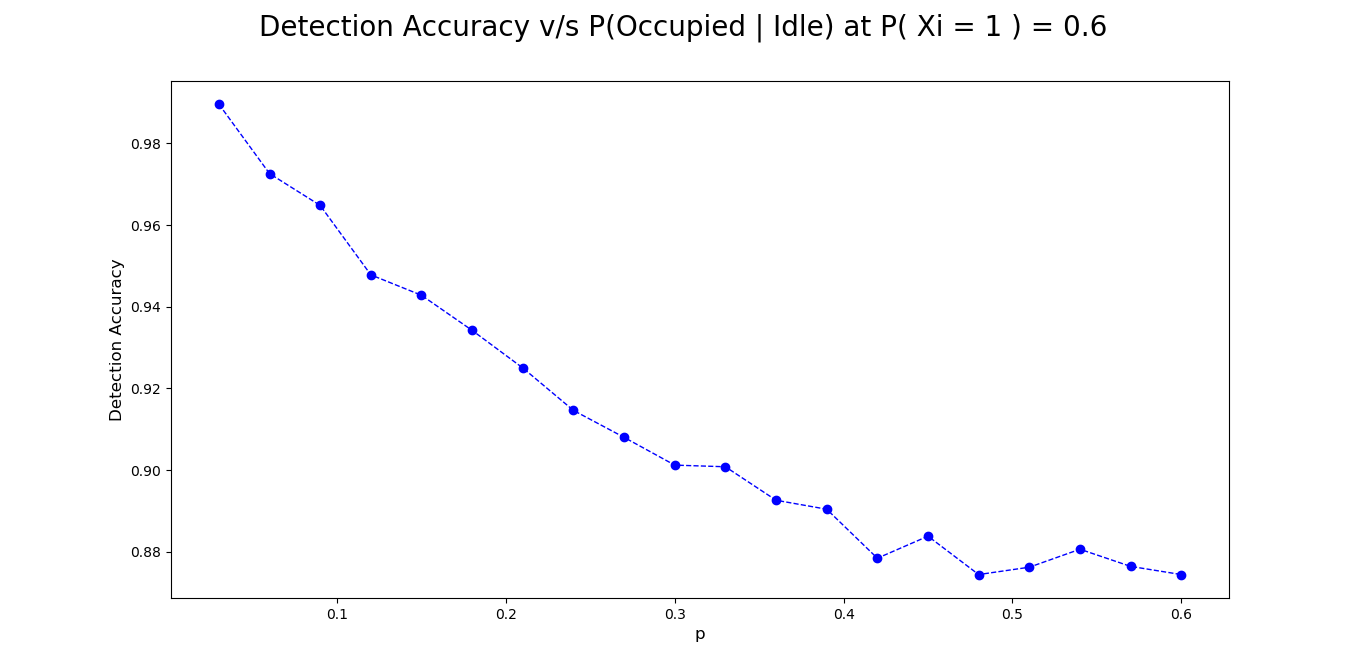
\includegraphics[width=1.0\textwidth]{DetectionAccuracy_v_p_test_3_final.png}
\caption{Detection Accuracy v/s p for $1000$ observations per band averaged over 50 independent trials with $\Pi\ =\ 0.60$ and $p$ varied from $0.03$ to $\Pi$. This plot corresponds to a linear noisy observation model with the system obviously modelled as an HMM. The true states for the 18 frequency bands are generated using a custom Markov state generator $\forall p\ and\ \forall q$ with a fixed $\Pi\ =\ 0.6$.}
\label{fig:mesh3}
\centering
\end{figure}
\clearpage
\section{Static PU with Channel Correlation and Incomplete Information}
\subsection{Observation Model}
\begin{equation}\label{28}
    Y_k(i) = H_kX_k(i) + V_k(i)
\end{equation}
where,
\\$i\ \in\ \{1,\ 2,\ 3,\ .........,\ T\}$ represents the index of the observation
\\\textbf{NOTE}: Multiple observations of all the frequency bands are made by the SU for training the algorithm and averaging the results over numerous iterations. However, the PU occupancy behavior in this case remains static over time.
\\$k\ \in\ \{1,\ 2,\ 3,\ .........,\ K\}$ represents the index of the sub-band
\\$V_k(i)\ \sim\ \mathcal{N}(0,\ \sigma_V^2)$ represents the zero-mean additive Gaussian noise sample
\\$H_k\ \sim\ \mathcal{N}(0,\ \sigma_H^2)$ represents the $k^{th}$ DFT coefficient of the impulse response $h(n)$ of the channel in between the PU and the SU receiver
\\The PU occupancy behavior in each sub-band $b_k\ \in\ B$ is modelled as $X_k$ taking two possible values $0\ and\ 1$. Therefore, the PU occupancy behavior in the entire wideband spectrum of interest discretized into narrow-band frequency components can be modelled as a vector of size $|B|\ =\ K$ such that,
\begin{equation}\label{29}
    \vec{X} = [X_1, X_2, X_3, ........., X_K]^T \in \{0,1\}^K
\end{equation}
\subsection{System Model}
The true states encapsulate the actual behavior of the PU which is an unobserved Markov process and the measurements at the SU are noisy observations of the true states which are modelled to be the observed states of a Hidden Markov Model.
For some sub-band $j\ \in\ \{2,\ 3,\ 4,\ .....,\ K\}$, the system is assumed to satisfy the Markov property as shown below,
\[P(X_{j}(i)|X_{j-1}(i),\ X_{j-2}(i),\ .....,\ X_1(i))\ =\ P(X_{j}(i)|X_{j-1}(i)),\ for\ j>1,\]
\[And,\ we\ will\ use\ P(X_1(i))\ for\ j=1.\]
Since \textbf{the PU is assumed to be static in the period of our estimation}, we can write the above assumption as,
\[P(X_{j}|X_{j-1},\ X_{j-2},\ .....,\ X_1)\ =\ P(X_{j}|X_{j-1}),\ for\ j>1,\]
\[And,\ we\ will\ use\ P(X_1)\ for\ j=1.\]
Now, we know that,
\[\vec{X}\ =\ [X_1,\ X_2,\ X_3,\ ......,\ X_K]^T\] which realizes as,
\[\vec{x}\ =\ [x_1,\ x_2,\ x_3,\ ......,\ x_K]^T\]
So,
\begin{equation}\label{30}
    P(\vec{X}=\vec{x}) = P(X_1=x_1) \prod_{k=2}^{K} P(X_k=x_k|X_{k-1}=x_{k-1})
\end{equation}
\textbf{Assuming there is a single PU and a single SU making observations}, we have, from the observation model,
\begin{equation}\label{31}
    P(Y_k|X_k = x_k)\ \sim \mathcal{N}(0,\ \sigma_H^2x_k+\sigma_V^2)
\end{equation}
In this extension, the SU does not sense all $|B|\ =\ K$ frequency bands in the wideband spectrum of interest. Instead, a subset $M\ <\ K$ frequency bands are sensed based on recommendations given a Bandit or a Reinforcement Learning agent. Let the set of these "incomplete" observations be given as,
\[\vec{Y}\ =\ [y_1,\ y_2,\ \phi,\ ...,\ \phi,....,\ y_m,\ \phi,\ ...,\ y_K]^T\]
where, $\vec{Y}$ represents the observation vector with $\phi$ filled in for frequency bands which have not been observed.
Based on this System Model and Observation Model, the state sequence estimation procedure detailed in Section 1 (\textit{Static PU with complete observations}) can be modified to account for missing observations as described in Section 2.3.
\subsection{The Estimator}
Assuming a static PU across time, a linear, noisy observation model, and a Markovian correlation across the frequency channels, the optimization problem can be stated as follows.
\begin{equation}\label{32}
    \vec{x}^* = argmax_{\vec{x}} P(\vec{X}|\vec{Y})
\end{equation}
\[\vec{x}^* = argmax_{\vec{x}} P(\vec{X}\ =\ [x_1,\ x_2,\ x_3,\ ......,\ x_K]^T\ |\ \vec{Y}\ =\ [y_1,\ y_2,\ \phi,\ ...,\ \phi,....,\ y_m,\ \phi,\ ...,\ y_K]^T)\]
For $X_1 = x_1$, i.e. \textbf{Initialization},
\[V_1^{(r)}\ =\ m_r(y_1)\pi_r,\ if\ y_1\ \neq\ \phi\]
\[V_1^{(r)}\ =\ \pi_r,\ if\ y_1\ = \phi\]
where,
\[m_r(y_1)\ \sim \mathcal{N}(0,\ \sigma_H^2r+\sigma_V^2),\]
\[\pi_r\ \in\ \Pi\ ,\ and\]
\[r\ \in\ \{0,\ 1\}\]
Now, moving on to the \textbf{Forward Recursion aspect},
\[V_j^{(r)}\ =\ m_r(y_j)\ max_l[a_{lr}V_{j-1}^{(l)}],\ if\ y_j\ \neq\ \phi\]
\[V_j^{(r)}\ =\ max_l[a_{lr}V_{j-1}^{(l)}],\ if\ y_j\ =\ \phi\]
where,
\[m_r(y_j)\ \sim \mathcal{N}(0,\ \sigma_H^2r+\sigma_V^2),\]
\[j\ \in\ \{2,\ 3,\ 4,\ ......,\ K\}\]
\[l,\ r\ \in\ \{0,1\}\]
Now, moving on to the \textbf{Backtracking aspect},
\[Ptr_j\ =\ argmax_l(a_{lr}V_{j-1}^{(l)})\]
\[k^*\ =\ argmax_k(V_K^{(k)})\]
\[x_{i-1}^*\ =\ Ptr_i\]
There are other approaches to this "missing observations" problem of state estimation. For example, approaches like Gluing and Multi-sequences are discussed in Ref [\ref{10}]. Similar models are used in Automatic Speech Recognition with Missing Data (ASR with MD) as detailed in Ref [\ref{11}].
\section{Dynamic PU with Temporal Correlation and Channel Correlation with Complete Information}
\subsection{Observation Model}
Persisting the same observation model as in the previous sections,
\begin{equation}\label{33}
    Y_k(i) = H_kX_k(i) + V_k(i)
\end{equation}
where,
\\$i\ \in\ \{1,\ 2,\ 3,\ .........,\ T\}$ represents the index of the observation
\\$k\ \in\ \{1,\ 2,\ 3,\ .........,\ K\}$ represents the index of the sub-band
\\$V_k(i)\ \sim\ \mathcal{N}(0,\ \sigma_V^2)$ represents the zero-mean additive Gaussian noise sample
\\$H_k\ \sim\ \mathcal{N}(0,\ \sigma_H^2)$ represents the $k^{th}$ DFT coefficient of the impulse response $h(n)$ of the channel in between the PU and the SU receiver
\\The PU occupancy behavior in each sub-band $b_k\ \in\ B$ is modelled as $X_k$ taking two possible values $0\ and\ 1$. Therefore, the PU occupancy behavior in the entire wideband spectrum of interest discretized into narrow-band frequency components can be modelled as a vector of size $|B|\ =\ K$ such that,
\begin{equation}\label{34}
    \vec{X} = [X_1, X_2, X_3, ........., X_K]^T \in \{0,1\}^K
\end{equation}
Solving for the mean and variance of $Y_k(i)$ from (\ref{33}) with $X_k(i)\ =\ x_k$, we get,
\begin{equation}\label{35}
    E[Y_k(i) | X_k(i) = x_k] = 0
\end{equation}
\begin{equation}\label{36}
    Var[Y_k(i) | X_k(i) = x_k] = \sigma_H^2x_k + \sigma_V^2
\end{equation}
Therefore,
\[Y_k(i)\ \sim\ \mathcal{N}(0,\ \sigma_H^2x_k + \sigma_V^2)\]
\subsection{System Model}
The system model comprises a \textbf{2D Markov Chain: one across time and one across frequency bands - all the frequency bands in the wideband spectrum of interest are sensed by the SU in each sampling round $t$}. We'll see the next extension of this work (PU Occupancy Behavior Estimation with Time and Channel Markovian Correlation and Incomplete Information) in Section 4 of this document.
\\The \textbf{transition probabilities matrix} for PU Occupancy Behavior transitions, i.e $0\longrightarrow1$ or $1\longrightarrow0$ across both time and frequency is given by,
\[A\ =\ [a_{mnr}]\ such\ that\ a_{mnr}\ =\ P(x_{tk}\ =\ r\ |\ x_{t-1,k}\ =\ m,\ x_{t,k-1}\ =\ n]\]
where,
\[r,\ m,\ n\ \in\ \{0,1\}\ represents\ the\ PU\ occupancy\ state\ in\ a\ particular\ channel\ at\ a\ particular\ time\]
\[t\ \in\ \{2,\ 3,\ 4,\ .....,\ T\}\ represents\ the\ temporal\ index\]
\[k\ \in\ \{2,\ 3,\ 4,\ .....,\ K\}\ represents\ the\ channel\ index\]
From the observation model, the \textbf{emission probabilities} are given by,
\[m_r(y_{tk})\ =\ P(y_{tk}\ |\ x_{tk}\ =\ r)\ \sim\ \mathcal{N}(0,\ \sigma_H^2r+\sigma_V^2)\]
where,
\[r\ \in\ \{0,1\}\]
The \textbf{initial or start probabilities} are given as follows.
\[\Pi\ =\ \{\pi_r:\ \pi_r\ =\ P(x_{tk}\ =\ r)\ for\ t\ =\ 1\ or\ k\ =\ 1,\ \forall\ r\ \in\ \{0,1\}\}\]
\subsection{Visualization of Temporally and Spatially Correlated PU behavior}
The following visualization results illustrate the Occupancy Behavior of the Primary User in a wideband spectrum of interest consisting of 18 frequency bands observed over 100 sampling rounds. The PU behavior is dynamic (varying across time).
\begin{itemize}
    \item Figure 4 depicts the PU Occupancy Behavior across time indices (sampling rounds) and across channel indices (frequency bands) assuming that a dual Markov chain exists- one across channels and one across sampling rounds. Mathematical details about the System Model are outlined in the previous subsection. Specifically, for both the Markov chains, 
    \[P(Occupied|Idle)\ =\ P(X_j = 1|X_i = 0)\ =\ p\ =\ 0.3\]
    \[P(Occupied)\ =\ P(X_i\ =\ 1)\ =\ \Pi\ =\ 0.6\]
    \item Figure 5 depicts the PU Occupancy Behavior across time indices (sampling rounds) and across channel indices (frequency bands) assuming independence among channels and among sampling rounds, i.e,
    \[P(Occupied|Idle)\ =\ P(X_j = 1|X_i = 0)\ =\ p\ =\ P(Occupied)\ =\ P(X_i\ =\ 1)\ = \Pi\ =\ 0.3\]
\end{itemize}
\begin{figure}[t]
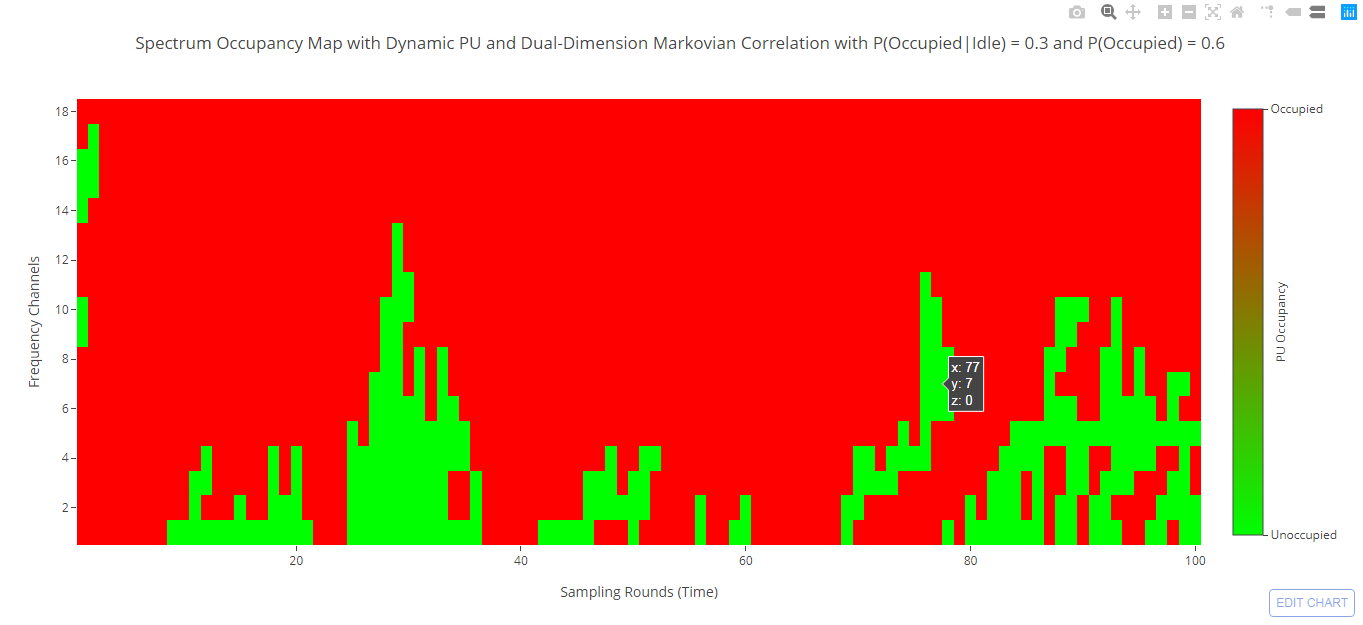
\includegraphics[width=1.0\textwidth]{Spectrum_Occupancy_HeatMap_Dynamic_SpatioTemporal_Corr.png}
\caption{Dynamic PU Occupancy Behavior with Markovian Correlation across channel indices and across time indices}
\label{fig:mesh4}
\centering
\end{figure}
\begin{figure}[t]
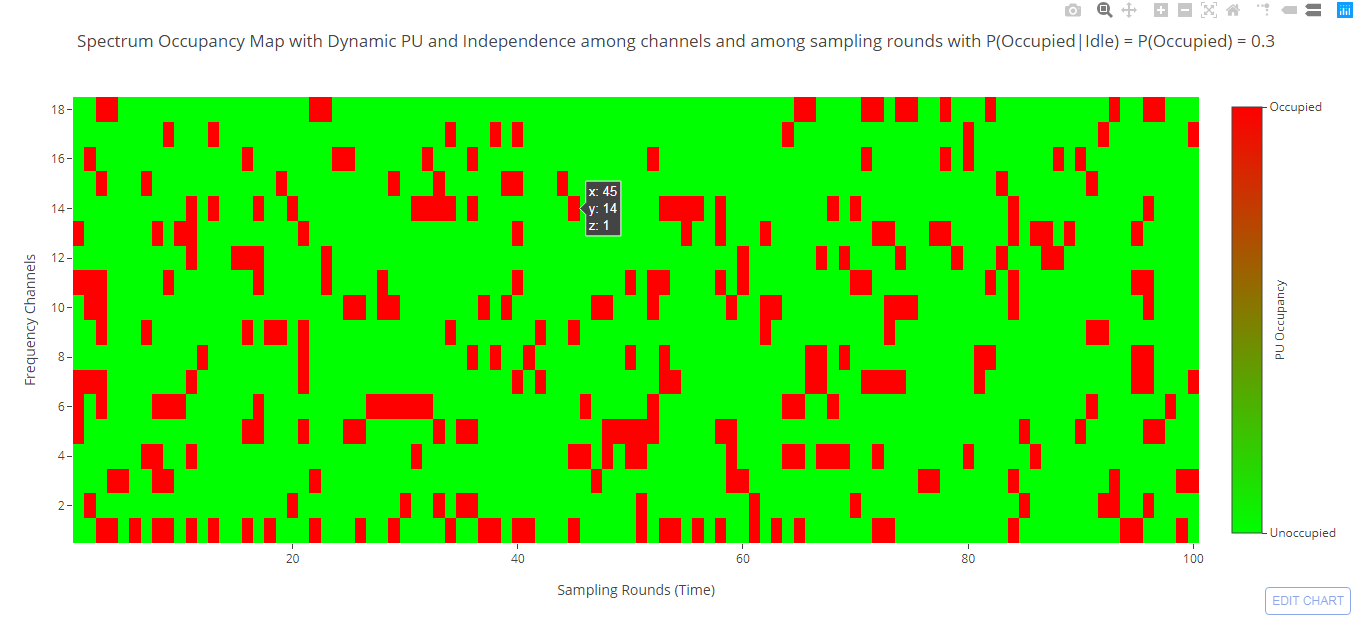
\includegraphics[width=1.0\textwidth]{Spectrum_Occupancy_HeatMap_Dynamic_Independence.png}
\caption{Dynamic PU Occupancy Behavior with independence among channels and among sampling rounds}
\label{fig:mesh5}
\centering
\end{figure}
\subsection{The Estimator}
\subsubsection{Notations}
Let us first define the notations employed in this analytical derivation.
\\The set of all past observations required for the estimation of PU Occupancy in channel $k$ in sampling round $t$ is given as follows.
\[y_{1:t-1,1:k-1}\ =\ \{y_{t,1},y_{t,2},...,y_{t,k-1},y_{1,k},y_{2,k},...,y_{t-1,k}\}\]
\\The set of all past states required for the estimation of PU Occupancy in channel $k$ in sampling round $t$ is given as follows.
\[x_{1:t-1,1:k-1}\ =\ \{x_{t,1},x_{t,2},...,x_{t,k-1},x_{1,k},x_{2,k},...,x_{t-1,k}\}\]
\\The joint probability term while analyzing state-observation pair of channel $k$ which is in state $r \in \{0,1\}$ in sampling round $t$ is denoted as follows.
\[P(y_{tk}, x_{tk}=r, y_{1:t-1,1:k-1}, x_{1:t-1,1:k-1})\]
The probability terms are simplified and the estimation algorithm's analytical expressions are derived in the upcoming subsubsections.
\subsubsection{Defining the Probability terms}
The joint probability term for analyzing the state-observation pair of channel $k$ which is in state $r \in \{0,1\}$ in sampling round $t$ is defined as follows. Note that, channel $k$ is in state $m \in \{0,1\}$ in sampling round $t-1$ and channel $k-1$ is in state $n \in \{0,1\}$ in sampling round $t$. Based on our System Model described subsection B of section III, the PU Occupancy state at location $(t,k)$ depends only on the PU Occupancy states at locations $(t-1,k)$ and $(t,k-1)$ respectively, i.e. the previous states both temporally and spatially.
\begin{equation*}
    P(y_{tk}, x_{tk}=r, y_{1:t-1,1:k-1}, x_{1:t-1,1:k-1})
\end{equation*}
Using the definition of conditional probability, the joint probability term from above can be written as,
\begin{equation*}
    P(y_{tk}, x_{tk}=r|y_{1:t-1,1:k-1}, x_{1:t-1,1:k-1})P(y_{1:t-1,1:k-1}, x_{1:t-1,1:k-1})
\end{equation*}
Using the Markov property across both time indices (sampling rounds or iterations) and channel indices, the joint probability term from above can be written as,
\begin{equation*}
    P(y_{tk}, x_{tk}=r|x_{t-1,k}=m,x_{t,k-1}=n)P(y_{1:t-1,1:k-1}, x_{1:t-1,1:k-1})
\end{equation*}
Simplifying the conditional even further, the aforementioned joint probability term can be written as,
\begin{equation*}
        P(y_{tk}|x_{tk}=r,x_{t-1,k}=m,x_{t,k-1}=n)P(x_{tk}=r|x_{t-1,k}=m,x_{t,k-1}=n)P(y_{1:t-1,1:k-1}, x_{1:t-1,1:k-1})
\end{equation*}
Since the observations depend only on the current state, the joint probability term can be further simplified as,
\begin{equation*}
        P(y_{tk}|x_{tk}=r)P(x_{tk}=r|x_{t-1,k}=m,x_{t,k-1}=n)P(y_{1:t-1,1:k-1}, x_{1:t-1,1:k-1})
\end{equation*}
Using the definitions of emission and state transition probabilities from the System Model, the aforementioned joint probability term can be written as,
\begin{equation*}
        m_r(y_{tk})a_{mnr}P(y_{1:t-1,1:k-1}, x_{1:t-1,1:k-1})
\end{equation*}
\subsubsection{Maximization of the Probabilities to arrive at the Forward and Backward Variables}
For the state estimation analysis, let's derive the analytical equations for a state element $x_{tk}\ =\ r$ and for the corresponding observation element $y_{tk}$. We'll now derive the forward and backward variables based on this \textit{node} and it's neighbors.
Let us first define the value function $V_{t-1,k-1}^{(l)}$ as follows.
\begin{equation}\label{37}
        V_{t-1,k-1}^{(l)}\ =\ max_{1:t-2,1:k-2}[P(y_{1:t-2,1:k-2},x_{1:t-2,1:k-2},y_{t-1,k-1},x_{t-1,k-1}=l)]
\end{equation}
Here, $V_{t-1,k-1}^{(l)}$ represents the maximum probability of emission of $y_{t-1,k-1}$ with $x_{t-1,k-1}\ =\ l\ \in\ \{0,1\}$.
\\Now, since we have two dimensions (time indices and channel indices) in our System Model, we will have two flavors of value functions as discussed below. Let's first define $V_{t-1,k}^{(m)}$, i.e. the \textbf{horizontal transition across channel indices} with respect to $ V_{t-1,k-1}^{(l)}$ in the same way as in equation (\ref{37}).
\begin{equation}\label{38}
   V_{t-1,k}^{(m)}\ =\ max_{1:t-2,1:k-1}[P(y_{1:t-2,1:k-1},x_{1:t-2,1:k-1},y_{t-1,k},x_{t-1,k}=m)]
\end{equation}
Similarly, let's define the value functions for time index traversal as follows.
Writing $V_{t,k-1}^{(n)}$, i.e. the \textbf{vertical transition across time indices} with respect to $ V_{t-1,k-1}^{(l)}$ in the same way as in equation (\ref{37}),
\begin{equation}\label{39}
    \begin{aligned}
        V_{t,k-1}^{(n)}\ =\ max_{1:t-1,1:k-2}[P(y_{1:t-1,1:k-2},x_{1:t-1,1:k-2},y_{t,k-1},x_{t,k-1}=n)]
    \end{aligned}
\end{equation}
Now, let's define the \textbf{Forward Recursion} Value function for $V_{tk}^{(r)}$ using the analytical equations defined above.
From equation (\ref{37}),
\begin{equation}\label{40}
         V_{t,k}^{(r)}\ =\ max_{1:t-1,1:k-1}[P(y_{1:t-1,1:k-1}, x_{1:t-1,1:k-1},y_{tk},x_{tk}=r)]
\end{equation}
Now, using the definition of conditional probability, we have,
\begin{equation}\label{41}
    V_{t,k}^{(r)}\ =\ max_{1:t-1,1:k-1}[P(y_{tk}, x_{tk}=r|y_{1:t-1,1:k-1}, x_{1:t-1,1:k-1})P(y_{1:t-1,1:k-1}, x_{1:t-1,1:k-1})]
\end{equation}
Since, we have a Markovian correlation across both time and frequency, we can apply the Markov property to equation (\ref{41}), to get,
\begin{equation}\label{42}
         V_{t,k}^{(r)}\ =\ max_{1:t-1,1:k-1}[P(y_{tk}, x_{tk}=r|x_{t-1,k}=m,x_{t,k-1}=n)P(y_{1:t-1,1:k-1}, x_{1:t-1,1:k-1})]
\end{equation}
Simplifying the conditional even further, we have,
\begin{equation}\label{43}
\begin{aligned}
    V_{t,k}^{(r)}\ =\ max_{1:t-1,1:k-1}[P(y_{tk}|x_{tk}=r,x_{t-1,k}=m,x_{t,k-1}=n)P(x_{tk}=r|x_{t-1,k}=m,x_{t,k-1}=n)\\P(y_{1:t-1,1:k-1}, x_{1:t-1,1:k-1})]
\end{aligned}
\end{equation}
Since the observation in location $(t,k)$ depends only on the PU Occupancy state $x_{t,k}\ =\ r \in \{0,1\}$,
\begin{equation}\label{44}
    V_{t,k}^{(r)}\ =\ max_{1:t-1,1:k-1}[P(y_{tk}|x_{tk}=r)P(x_{tk}=r|x_{t-1,k}=m,x_{t,k-1}=n)P(y_{1:t-1,1:k-1}, x_{1:t-1,1:k-1})]
\end{equation}
From the system model definitions of emission and transition probabilities, equation (\ref{44}) can be written as,
\begin{equation}\label{45}
    V_{t,k}^{(r)}\ =\ m_r(y_{tk})\ max_{1:t-1,1:k-1}[a_{mnr}P(y_{1:t-1,1:k-1}, x_{1:t-1,1:k-1})]
\end{equation}
Factorizing the joint distribution into its independent constituent marginals and splitting the maximization operator, we have,
\begin{equation}\label{46}
    \begin{aligned}
         V_{t,k}^{(r)}\ =\ m_r(y_{tk})\ max_{(t,k-1),(t-1,k)}[a_{mnr}\  max_{1:k-1}[P(y_{1:k-2},x_{1:k-1})]max_{1:t-1}[P(y_{1:t-1},x_{1,t-1})]]
    \end{aligned}
\end{equation}
Using redundancy, equation (\ref{46}) can be written as,
\begin{equation}\label{47}
    \begin{aligned}
         V_{t,k}^{(r)}\ =\ m_r(y_{tk})\ max_{m,n}[a_{mnr}max_{1:k-2,1:t-1}[P(y_{1:k-2},y_{t,k-1},y_{1:t-1},x_{1:k-2},x_{t,k-1}=n,x_{1:t-1})]\\max_{1:t-2,1:k-1}[P(y_{1:t-2},y_{t-1,k},y_{1:k-1},x_{1:t-2},x_{t-1,k}=m,x_{1:k-1})]]]
    \end{aligned}
\end{equation}
Consolidating terms inside the joint probabilities, we have,
\begin{equation}\label{48}
    \begin{aligned}
         V_{t,k}^{(r)}\ =\ m_r(y_{tk})\ max_{m,n}[a_{mnr}max_{1:k-2,1:t-1}[P(y_{1:k-2,1:t-1},y_{t,k-1},x_{1:k-2,1:t-1},x_{t,k-1}=n)]\\max_{1:t-2,1:k-1}[P(y_{1:t-2,1:k-1},y_{t-1,k},x_{1:t-2,1:k-1},x_{t-1,k}=m)]]]
    \end{aligned}
\end{equation}
Now, we know from equations (\ref{38}) and (\ref{39}) that,
\begin{equation*}
   V_{t-1,k}^{(m)}\ =\ max_{1:t-2,1:k-1}[P(y_{1:t-2,1:k-1},x_{1:t-2,1:k-1},y_{t-1,k},x_{t-1,k}=m)]
\end{equation*}
\begin{equation*}
    V_{t,k-1}^{(n)}\ =\ max_{1:t-1,1:k-2}[P(y_{1:t-1,1:k-2},x_{1:t-1,1:k-2},y_{t,k-1},x_{t,k-1}=n)]
\end{equation*}
Using these results in equation (\ref{48}), we get,
\begin{equation}\label{49}
    \begin{aligned}
         V_{t,k}^{(r)}\ =\ m_r(y_{tk})max_{m,n}[a_{mnr}V_{t,k-1}^{(n)}V_{t-1,k}^{(m)}]
    \end{aligned}
\end{equation}
So, intuitively, the maximum probability of emission of $y_{tk}$ with the actual state of channel $k$ in sampling round $t$ depends on the previous element along the column vector (i.e. time) and the previous element along the row vector (i.e. channel) in addition to the probability of transitioning from $n \longrightarrow r$ horizontally and the probability of transitioning from $m \longrightarrow r$ vertically. The previous elements $(t,k-1)$ and $(t-1,k)$ depend on $V_{t-1,k-1}^{(l)}$.
\\Now, similar to the \textbf{backtracking procedure} in the 1D Viterbi algorithm, the Trellis diagram is traversed backwards from the final state to recover its two previous neighbors: one along the channel index and the other along the temporal index. This is done recursively until the entire Trellis has been traversed all the way back to the first state in the most probable state sequence (Viterbi path).
\\Mathematically,
\begin{equation}\label{50}
    \begin{aligned}
         x_{t-1,k-1}^*\ =\ l^*\ =\ argmax_{l}\{a_{mnr}\ V_{t,k-1}^{(n)}V_{t-1,k}^{(m)}\}
    \end{aligned}
\end{equation}
Using the analytical equations derived for both the \textbf{Forward Recursion phase and the Backtracking phase of our 2D Viterbi algorithm}, the final algorithm is given as follows.
\subsection{The Algorithm}
\begin{flushleft}
\textbf{Initialization}: The array of initial probabilities $\Pi$ is known.
\\\textbf{Forward Recursion}: $V_{t,k}^{(r)}\ =\ m_r(y_{tk})max_{m,n}[a_{mnr}V_{t,k-1}^{(n)}V_{t-1,k}^{(m)}]$
\\\textbf{Backtrack}: $x_{t-1,k-1}^{(r)*}\ =\ l^*\ =\ argmax_{l}\{a_{mnr}\ V_{t,k-1}^{(n)}V_{t-1,k}^{(m)}\}$
\\\textbf{Termination}: $P([y_{tk}]\ |\ [x_{tk}])\ =\ max_s\ V_{TK}^{(s)}$
\end{flushleft}
\textit{This will be implemented in Python and numerical results such as the $Detection\ Accuracy$ of our estimator will be reported}.
\section{Dynamic PU with Temporal Correlation and Channel Correlation with Incomplete Information}
In this extension, the SU does not sense all $|B|\ =\ K$ frequency bands in the wideband spectrum of interest. Instead, a subset $M\ <\ K$ frequency bands are sensed in a given sampling round based on recommendations given a Bandit or a Reinforcement Learning agent. Let the set of these "incomplete" observations in sampling round $t$ be given as,
\[\vec{Y}_t\ =\ [y_{t,1},\ y_{t,2},\ \phi,\ ...,\ \phi,....,\ y_{t,m},\ \phi,\ ...,\ y_{t,K}]^T\]
where, $\vec{Y}_t$ represents the observation vector in sampling round $t$ with $\phi$ filled in for frequency bands which have not been observed.
Based on this System Model and Observation Model, the state sequence estimation procedure detailed in Section 3 (\textit{Dynamic PU behavior with complete observations}) can be modified to account for missing observations as described below.
Persisting the same observation model and system model as in the previous sections, we can write the \textbf{Forward Recursion} step and \textbf{Backtracking} step of the 2D Viterbi algorithm with missing observations as follows,
\[V_{t,k}^{(r)}\ =\ m_r(y_{tk})max_{m,n}[a_{mnr}V_{t,k-1}^{(n)}V_{t-1,k}^{(m)}],\ if\ y_{tk}\neq\phi\]
\[V_{t,k}^{(r)}\ =\ max_{m,n}[a_{mnr}V_{t,k-1}^{(n)}V_{t-1,k}^{(m)}],\ if\ y_{tk}=\phi\]
\[x_{t-1,k-1}^*\ =\ l^*\ =\ argmax_{l}\{a_{mnr}\ V_{t,k-1}^{(n)}V_{t-1,k}^{(m)}\}\]
\section{External References}
\begin{enumerate}
    \item \textbf{Fast Spectrum Sensing: A Combination of Channel Correlation and Markov Model}: https://ieeexplore.ieee.org/document/6956794
    \item \textbf{Factorial Hidden Markov Models}:\newline http://www.ee.columbia.edu/~sfchang/course/svia-F03/papers/factorial-HMM-97.pdf
    \item \textbf{Coupled Hidden Markov Models for complex action recognition}:\newline http://www.ee.columbia.edu/~sfchang/course/svia-F03/papers/brand96coupled-hmm.pdf
    \item \textbf{Modeling Temporal Activity Patterns in Dynamic Social
    Networks}: \\https://arxiv.org/pdf/1305.1980.pdf
    \item \textbf{HMM based Channel Status Predictor for Cognitive Radio}: In this work, the authors describe a Channel Set Management system which employs pre-loaded data from a database as the "Channel History". The system then uses the observations from this training data set to estimate the parameters of the HMM using the Baum-Welch algorithm. Furthermore, the next state of the channel is predicted using the Forward algorithm, although that is not clear in the paper as to how they do it. [\textit{https://ieeexplore.ieee.org/document/4554696}]
    \item \textbf{A State Action Frequency Approach to Throughput Maximization over Uncertain Wireless Channels}: In this paper, the authors model wireless channels as finite parallel queues which individually evolve as an independent ON/OFF Markov chain. No CSI is assumed. Instead, this work proposes an ACK-feedback mechanism to update the success of transmission \textit{a posteriori}. Then, the paper goes on to talk about optimal scheduling policies for fully backlogged systems by using tools from MDP theory and Queueing Theory.\newline
    [\textit{https://ieeexplore.ieee.org/document/5935211/}]
    \item \textbf{Joint Spectral-Temporal Spectrum Prediction from Incomplete Historical Observations}: In this work, the authors analyze the temporal and spectral correlation that exists in the data-sets gathered in a spectrum database stored in a secondary base station operating in an IEEE 802.22 WRAN radio ecosystem, using correlation coefficients. Furthermore, the authors go on to describe a data driven joint spectral temporal spectrum prediction approach by modelling the problem of having incomplete observations as a matrix completion problem (fill in the missing entries of the spectrum data matrix).\newline
    [\textit{https://ieeexplore.ieee.org/abstract/document/7032338}]
    \item \textbf{Hidden Markov Model State Estimation with Randomly Delayed Observations}: In this paper, the authors discuss a state estimation technique for a discrete-time Hidden Markov Model when the observations are delayed by a random time. The proposal includes modelling the delay process as a finite state Markov chain and then reformulating the original HMM problem as an augmented HMM to model the whole system. State Estimation algorithms are then used for this reformulated HMM.\newline
    [\textit{https://ieeexplore.ieee.org/document/774757}]
    \item \textbf{A hidden semi-Markov model with missing data and multiple observation sequences for mobility tracking}: In this work, the authors propose the use of Ferguson's algorithm with modified Forward and Backward variables in order to account for missing observations in the formulated HSMM problem. They also propose numerous modifications to the state and parameter estimation algorithms in order to reduce their computational complexity.
    [\textit{https://dl.acm.org/citation.cfm?id=641933}]
    \item \textbf{A Comparison of Some Methods for Training Hidden Markov Models on Sequences with Missing Observations}: Here, the authors discuss numerous ways to solve state and parameter estimation for HMMs using the Marginalization approach, the Gluing approach, and the Multi-sequences approach. They also evaluate how the position of missing data in the sequence impacts the detection accuracy.\newline
    [\textit{https://ieeexplore.ieee.org/document/7884147}]
    \item \textbf{Robust Automatic Speech Recognition with Missing and Unreliable Data}: In this work, the authors detail the analyses of Marginalization and Imputation approaches to solving the state and parameter estimation problem in HMMs with missing and/or unreliable data in the domain of Automatic Speech Recognition.\newline
    [\textit{https://pdfs.semanticscholar.org/990c/f303416374d8df2b8b96d6dcffcb5ada666c.pdf}]
    \item \textbf{Spectral expansion solution for a class of Markov models: application and comparison with the matrix geometric method}: This work details the Spectral Expansion method for solving two dimensional Markov chains whose state space is finite in one dimension and infinite in the other. The spectral expansion method is applied in the context of M/M/N queueing systems with general breakdowns and repairs.\newline
    [\textit{https://www.sciencedirect.com/science/article/pii/016653169400025F}]
    \item \textbf{Hidden Markov Models for two-dimensional data}: 2D HMM solutions for pattern recognition in image processing.\newline
    [\textit{$https://link.springer.com/chapter/10.1007/978-3-319-00969-8_14$}]
    \item \textbf{A General Two-Dimensional Hidden Markov Model and its application in Image Classification}: A 2D Viterbi algorithm is proposed for applications in Aerial Image segmentation.\newline
    [\textit{https://ieeexplore.ieee.org/document/4379516}]
    \item \textbf{Image classification by a two-dimensional Hidden Markov Model}: The HMM parameters are estimated using the EM algorithm. A two-dimensional version of the Viterbi algorithm is developed to classify an image based on the trained HMM. Also, applications in aerial image segmentation are explored.\newline
    [\textit{https://ieeexplore.ieee.org/document/823977/}]
    \item \textbf{Approximate Viterbi Decoding for 2D-Hidden Markov Models}: A 2D Viterbi algorithm is developed for applications in handwriting recognition.\newline
    [\textit{https://ieeexplore.ieee.org/document/859261}]
\end{enumerate}
\end{document}
\bibliographystyle{IEEEtran}
\bibliography{IEEEabrv,ref}	
\end{document}